% ============================================================
% DIAGRAM: Recurrent Neural Network (Unrolled)
% ============================================================
% Caption: Figure 4.2: RNN unrolled through time.
%          (Adapted from Elman, 1991, p. 180)
% ============================================================

\documentclass[tikz,border=10pt]{standalone}
\usepackage{tikz}
\usepackage{amsmath}
\usepackage{amsfonts}

\usetikzlibrary{shapes,arrows,positioning,fit,calc,backgrounds}

\begin{document}

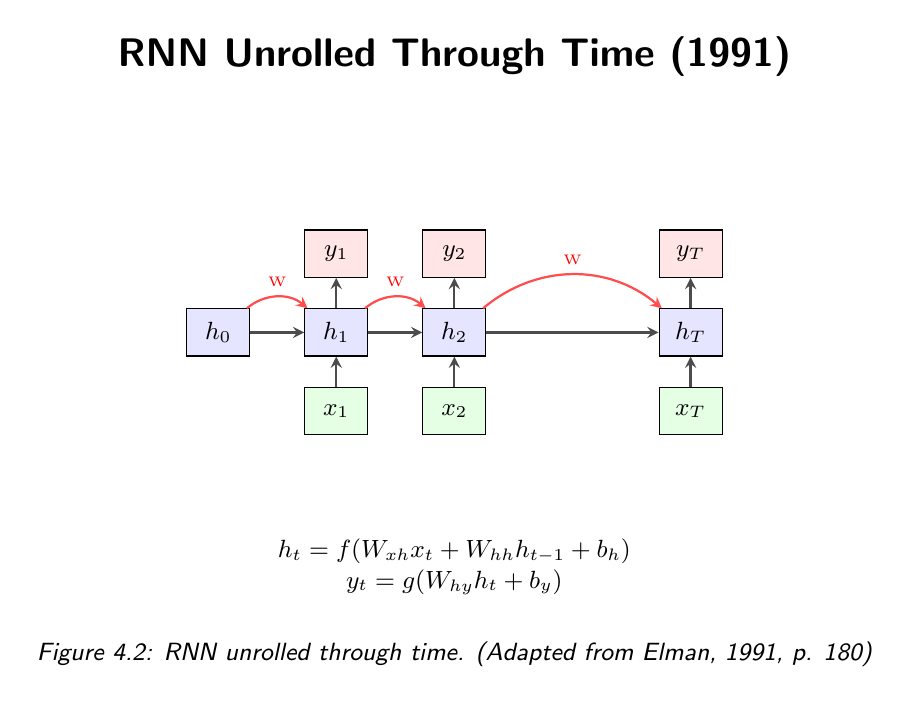
\begin{tikzpicture}[
    block/.style={draw, rectangle, minimum width=0.8cm, minimum height=0.6cm, fill=blue!10, font=\sffamily\small},
    edge/.style={-stealth, thick, draw=black!70},
    redge/.style={-stealth, thick, draw=red!70},
    label/.style={font=\sffamily\small},
    title/.style={font=\sffamily\Large\bfseries},
    caption/.style={font=\sffamily\small\itshape},
]

\node[title] at (0, 3.5) {RNN Unrolled Through Time (1991)};

% Time steps
\node[block] (h0) at (-3, 0) {$h_0$};
\node[block] (h1) at (-1.5, 0) {$h_1$};
\node[block] (h2) at (0, 0) {$h_2$};
\node[block] (hT) at (3, 0) {$h_T$};

% Inputs
\node[block, fill=green!10] (x1) at (-1.5, -1) {$x_1$};
\node[block, fill=green!10] (x2) at (0, -1) {$x_2$};
\node[block, fill=green!10] (xT) at (3, -1) {$x_T$};

% Outputs
\node[block, fill=red!10] (y1) at (-1.5, 1) {$y_1$};
\node[block, fill=red!10] (y2) at (0, 1) {$y_2$};
\node[block, fill=red!10] (yT) at (3, 1) {$y_T$};

% Edges
\draw[edge] (h0) -- (h1);
\draw[edge] (h1) -- (h2);
\draw[edge] (h2) -- (hT);

\draw[edge] (x1) -- (h1);
\draw[edge] (x2) -- (h2);
\draw[edge] (xT) -- (hT);

\draw[edge] (h1) -- (y1);
\draw[edge] (h2) -- (y2);
\draw[edge] (hT) -- (yT);

% Recurrent connections (highlighted)
\draw[redge, bend left=40] (h0) to node[above, font=\tiny, text=red] {W} (h1);
\draw[redge, bend left=40] (h1) to node[above, font=\tiny, text=red] {W} (h2);
\draw[redge, bend left=40] (h2) to node[above, font=\tiny, text=red] {W} (hT);

% Equation
\node[align=center, font=\sffamily\small, anchor=north] at (0, -2.5) {
  $h_t = f(W_{xh} x_t + W_{hh} h_{t-1} + b_h)$ \\
  $y_t = g(W_{hy} h_t + b_y)$
};

\node[caption, anchor=north] at (0, -3.8) {
  Figure 4.2: RNN unrolled through time. (Adapted from Elman, 1991, p. 180)
};

\end{tikzpicture}
\end{document}
